\documentclass{oci}
\usepackage[utf8]{inputenc}
\usepackage{lipsum}

\title{Bus de turismo}

\begin{document}
\begin{problemDescription}
  La empresa de turismo \emph{Al Sur del Mundo} tiene una flota de buses que
  utiliza para transportar a sus pasajeros en cada uno de los recorridos que
  ofrece a lo largo del país. 
  Todos los buses en la flota tienen 48 asientos distribuidos en 12 filas y con
  un pasillo de separación, tal como se muestra en la siguiente figura:
  \begin{center}
  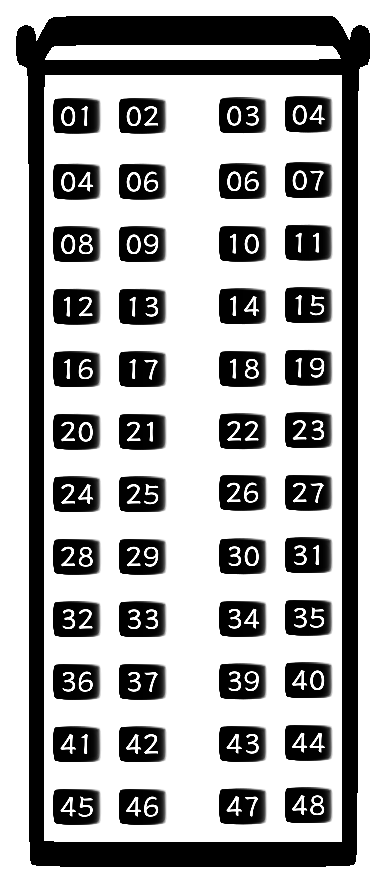
\includegraphics[scale=0.8]{bus.eps}
  \end{center}
  A menudo la gente hace reservas para grupos de más de una persona.
  Como es de esperar, a las personas siempre les gusta sentarse junto a alguien
  de su mismo grupo.
  Se considera que dos personas están juntas si están sentadas en la misma fila
  y no están separadas por el pasillo.
  A una persona que viaja sola nunca le importará dónde sentarse.

  Durante el último tiempo han surgido algunas inquietudes dentro de los
  directivos de la empresa, pues creen que mucha gente está quedando separada de
  su grupo, lo que estaría provocando mucha incomodidad entre los clientes.
  Los guías que trabajan directamente dentro de los buses creen que esto no es
  cierto pues ellos ayudan a los pasajeros a sentarse de forma óptima de modo
  que la máxima cantidad de pasajeros quede junto a alguien de su grupo.

  Dado el número de gente en cada grupo, y suponiendo que todos se sientan de
  forma óptima, tu tarea es determinar la cantidad de gente que no queda sentada
  junto a alguien de su grupo.
  
\end{problemDescription}

\begin{inputDescription}
  La primera línea de la entrada contiene un entero $N$ correspondiente a la
  cantidad de grupos que han hecho reserva.
  Cada una de las siguiente $N$ líneas contiene un entero mayor que cero
  correspondiente a la cantidad de gente en cada uno de los grupos.
  La cantidad total de gente nunca será mayor que 48.
\end{inputDescription}

\begin{outputDescription}
  La salida debe contener un único entero correspondiente a la cantidad de
  gente que \textbf{no} queda sentada junto a alguien de su grupo.
  A las personas que viajan solas no les importa dónde sentarse y por lo tanto
  no deben ser consideradas en esta cuenta.
\end{outputDescription}

\section*{Subtareas y puntaje}
Este problema no contiene subtareas.
Se probarán varios casos de prueba y se otorgará puntaje de acuerdo a la
cantidad de casos de prueba correctos.

\begin{sampleDescription}
\sampleIO{sample-1}
\sampleIO{sample-2}
\end{sampleDescription}

\end{document}